\documentclass[a4paper,12pt]{article}
% Math essential packages
\usepackage{latexsym, mathtools}
\usepackage{amsmath, amssymb, amsfonts, amsthm, amsxtra}
\usepackage[nomathsymbols]{polski}
\usepackage{amscd, tikz-cd}
\usepackage[skip=10pt, indent=0pt]{parskip}
\usepackage[a4paper, left=30mm, right=30mm, top=25mm, bottom=25mm]{geometry}
\usepackage{graphicx, float}
\usepackage{xcolor}
\usepackage[most,many,breakable]{tcolorbox}
\usepackage{relsize}
\usepackage{fancyhdr}
\usepackage{url}
\usepackage[colorlinks=true,citecolor=blue,urlcolor=blue,linkcolor=blue,pdfpagemode=UseNone]{hyperref}

\usepackage[framemethod=TikZ]{mdframed}
\usepackage{thmtools}

\usepackage{colortbl}
\usepackage{pgfplots}
\usepackage{subcaption}

\definecolor{accent}{RGB}{163,0,0}
\setlength{\arrayrulewidth}{0.2mm}
\renewcommand{\arraystretch}{1.2}

\usepackage{XCharter}

\title{Regresja Liniowa}
\author{Zachariasz Jażdżewski}
\date{18 maja 2024}

\begin{document}
\maketitle

%----Proper document------------------------------------------------------------

\section{Wprowadzenie}
Dzisiaj przedstawimy wam jedną z najważniejszych metod w nauce. Używaną w statystyce, analizie danych czy uczeniu maszynowym, którego używają takie systemy jak chociażby Chat GPT albo Midjourney. Wprowadzimy i zbadamy pojęcie regresji liniowej, ostaramy się zrozumieć czym intuicyjnie jest dopasowanie prostej oraz jak moglibyście samodzielnie opracować tą metodę od podstaw. Zacznijmy.

Rozważmy następujący problem: załóżmy, że zajmujemy się pomiarami dochodów i wydatków konsumpcyjnych w polskich rodzinach w przeliczeniu na osobę. Podczas pomiarów zebraliśmy takie dane:

\begin{table}[!h]
	\centering
	\begin{tabular}{ ccc }
		\hline
		\bfseries Indeks & \bfseries Dochody & \bfseries Wydatki \\ \hline
		1 & 200 & 120 \\
		2 & 250 & 190 \\
		3 & 285 & 200 \\
		4 & 300 & 270 \\
		5 & 350 & 285 \\
		6 & 395 & 320 \\
		7 & 440 & 340 \\
		8 & 490 & 340 \\
		9 & 510 & 390 \\
		10 & 530 & 410 \\
		\hline
	\end{tabular}
\end{table}

\newpage

Przedstawmy je na wykresie

\begin{figure}[h!]
	\centering
	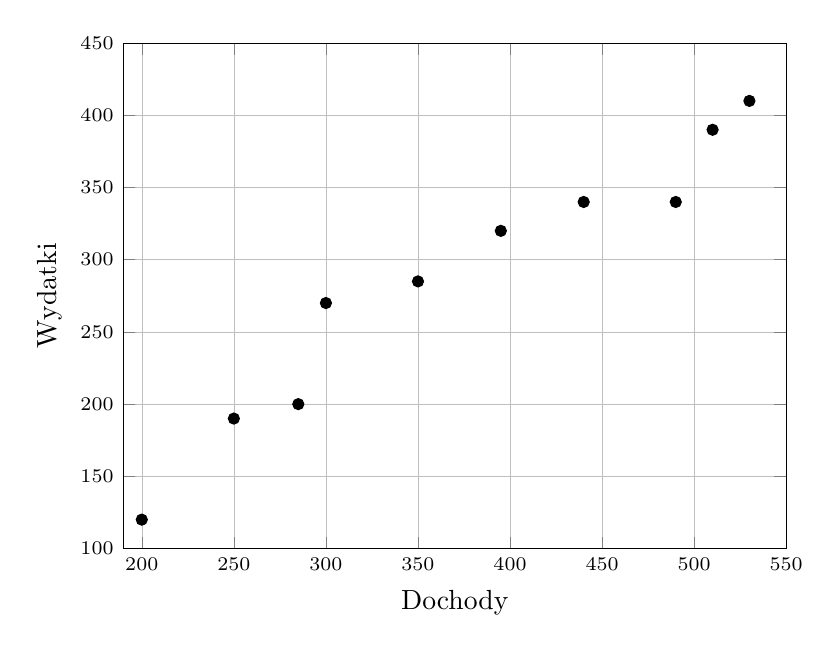
\begin{tikzpicture}
	\begin{axis}[
		xlabel={Dochody},
		ylabel={Wydatki},
		ymin=100, ymax=450,
		xmin=190, xmax=550,
		xtick={200,250,300,350,400,450,500,550},
		ytick={0,50,100,150,200,250,300,350,400,450},
		grid=both,
		grid style={line width=.1pt, draw=gray!10},
		major grid style={line width=.2pt,draw=gray!50},
		width=10cm,
		height=8cm,
		tick label style={font=\scriptsize}
	]
	\addplot[
		only marks,
		mark=*,
		]
		coordinates {
		(200,120) (250,190) (285,200) (300,270) (350,285) (395,320) (440,340) (490,340) (510,390) (530,410)
		};
	\end{axis}
	\end{tikzpicture}
\end{figure}

Mamy zatem $n = 10$ obserwacji, które przedstawiamy na płaszczyźnie jako punkty
\[
	(x_i, y_i) \in \{(200,120),(250,190),...,(530,410)\}, \quad i = 1,2,...,n
\]

Chcielibyśmy opisać ich wzajemną relację. Sądząc po rysunku możemy ocenić, że istnieje pozytywna korelacja między dochodami, a wydatkami. Przydatne byłoby jednak wiedzieć, jak silna jest ta zależność, moglibyśmy nawet na tej podstawie przewidywać jak zachowują się wydatki dla rodzin o niższych/wyższych dochodach. Aby to osiągnąć, musimy dopasować do danych taką krzywą $y$  która najlepiej będzie je reprezentować.

Jak mogliśmy zaobserwować na rysunku, punkty na płaszczyźnie układają się wzdłuż pewnej prostej,więc dla naszego przykładu możemy założyć, że krzywa jaką chcemy dopasować będzie krzywą liniową $y = ax+b$. Takich krzywych jest jednak nieskończenie wiele, jak zatem wybrać spośród nich taką, która najlepiej będzie modelowała nasze dane?Do tego potrzebujemy przyjąć pewne założenia. Co to w ogóle znaczy, że funkcja “najlepiej pasuje do zestawu danych”? ` x2`

\newpage

Na wykresie przedstawiliśmy 4 przykładowe proste. Która prosta jest z nich najlepsza? Dlaczego jest lepsza od innych? Jak możemy to sprawdzić?

\begin{figure}[h!]
	\centering
	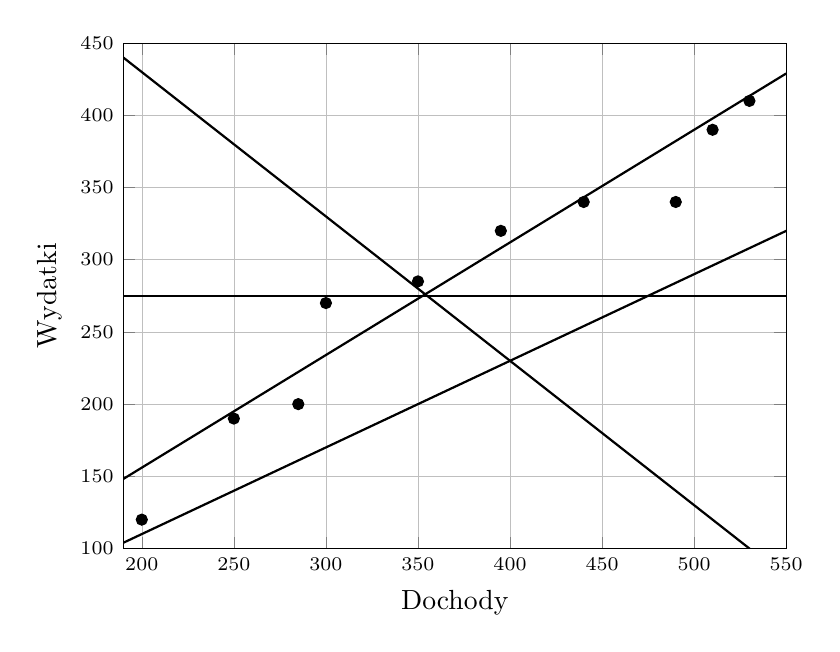
\begin{tikzpicture}
	\begin{axis}[
		xlabel={Dochody},
		ylabel={Wydatki},
		ymin=100, ymax=450,
		xmin=190, xmax=550,
		xtick={200,250,300,350,400,450,500,550},
		ytick={0,50,100,150,200,250,300,350,400,450},
		grid=both,
		grid style={line width=.1pt, draw=gray!10},
		major grid style={line width=.2pt,draw=gray!50},
		width=10cm,
		height=8cm,
		tick label style={font=\scriptsize}
	]
	\addplot[
		only marks,
		mark=*,
		]
		coordinates {
		(200,120) (250,190) (285,200) (300,270) (350,285) (395,320) (440,340) (490,340) (510,390) (530,410)
		};
	\addplot[
		domain=190:550, 
		samples=100, 
		thick
	]{-x + 630};
	\addplot[
		domain=190:550, 
		samples=100, 
		thick
	]{275};
	\addplot[
		domain=190:550, 
		samples=100, 
		thick
	]{0.6*x - 10};
	\addplot[
		domain=190:550, 
		samples=100, 
		thick
	]{0.78*x};
	\end{axis}
	\end{tikzpicture}
\end{figure}

Teoretycznie moglibyśmy oceniać czy dana funkcja liniowa pasuje do naszych danych “na oko”. Takie podejście jest jednak subiektywne i mało wydajne w przypadku bardziej skomplikowanych zestawów danych. Potrzebujemy zatem jakiejś obiektywnej metody, dzięki której dałoby się numerycznie wyznaczyć taką funkcję dla dowolnych zbiorów danych. 
Najstarszą i najbardziej powszechną taką metodą jest “metoda najmniejszych kwadratów” opracowana przez Carla Friedriecha Gaussa. 

\section{Metoda najmniejszych kwadratów}
Polega ona na znalezieniu takiej prostej dla której błąd między prostą a punktami jest jak najmniejszy.Nasz model $y=ax+b$ zależy od nieznanych nam parametrów $a$ i $b$. Chcemy je dobrać (oszacować) tak, aby suma różnic między punktami, a szacowaną prostą była jak najmniejsza. ` x2`Różnice takie możemy zapisać jako
\[
	y_i - (\hat a x_i + \hat b)
\]

gdzie $y_i$ to wartości $y$ naszych danych, a $\hat a x_i + \hat b$ to szacowana dzięki szukanej prostej wartość w punkcie $x_i$. Parametry $\hat a$ i $\hat b$ nazywamy estymatorami, a różnice takie nazywamy resztami.Zatem im bliżej $\hat a$ i $\hat b$ są prawdziwym (szukanym) wartościom $a$ i $b$, tym bardziej nasza reszta (a zatem i suma wszystkich reszt) będzie bliższa zeru.

Mamy jednak jeden problem. Nasze reszty mogą być dodatnie ALE też i ujemne, więc suma wszystkich reszt może być bliska zeru nawet gdy poszczególne reszty zdecydowanie nie są bliskie zeru. Zamiast tego możemy więc rozpatrywać reszty podniesione do kwadratu. To eliminuje nam problem kasowania się dodatnich i ujemnych reszt, jako, że wszystkie kwadraty reszt będą nieujemne.Wprowadza to nam jeszcze jeden bonus; kwadraty reszt z przedziału $(0,1)$ będą jeszcze mniejsze, a kwadraty większych reszt będą jeszcze większe, zatem jeszcze silniej będziemy minimalizować całą sumę.

Suma taka, dana wzorem
\[
	(y_1 - \hat a x_1 - \hat b)^2 + (y_2 - \hat a x_2 - \hat b)^2 + ... + (y_n - \hat a x_n - \hat b)^2 = \sum_{i=1}^n\,(y_i - \hat a x_i - b)^2
\]

będzie minimalna wtedy i tylko wtedy gdy każdy z kwadratów reszt będzie jak najmniejszy

Ustaliliśmy zatem obiektywny numeryczny wskaźnik, który pozwala nam na określenie, jak dobrze dopasowana jest dana linia do naszego zbioru danych. Sprawdźmy zatem dla paru przykładowych prostych ile wynosi suma kwadratów reszt dla naszego zestawu danych.

\begin{figure}[h!]
	\centering
	\begin{subfigure}[b]{0.45\textwidth}
		\centering
		\begin{tikzpicture}
		\begin{axis}[
			ymin=100, ymax=450,
			xmin=190, xmax=550,
			xtick={200,300,400,500},
			ytick={200,300,400},
			grid=both,
			grid style={line width=.1pt, draw=gray!10},
			major grid style={line width=.2pt,draw=gray!50},
			width=\textwidth,
			height=\textwidth,
			tick label style={font=\tiny}
		]
		\addplot[
			only marks,
			mark=*,
			]
			coordinates {
			(200,120) (250,190) (285,200) (300,270) (350,285) (395,320) (440,340) (490,340) (510,390) (530,410)
			};
		\addplot[
			domain=190:550, 
			samples=100, 
			thick
			]{0.66*x+30};
		\node[anchor=north east] at (axis cs:550,180) {$y = \frac{2}{3}x + 30$};
		\end{axis}
		\end{tikzpicture}
	\end{subfigure}%
	\begin{subfigure}[b]{0.45\textwidth}
		\centering
		\begin{tikzpicture}
		\begin{axis}[
			ymin=100, ymax=450,
			xmin=190, xmax=550,
			xtick={200,300,400,500},
			ytick={200,300,400},
			grid=both,
			grid style={line width=.1pt, draw=gray!10},
			major grid style={line width=.2pt,draw=gray!50},
			width=\textwidth,
			height=\textwidth,
			tick label style={font=\tiny}
		]
		\addplot[
			only marks,
			mark=*,
			]
			coordinates {
			(200,120) (250,190) (285,200) (300,270) (350,285) (395,320) (440,340) (490,340) (510,390) (530,410)
			};
		\addplot[
			domain=190:550, 
			samples=100, 
			thick
			]{0.5*x+100};
		\node[anchor=north east] at (axis cs:550,180) {$y = \frac{1}{2}x + 100$};
		\end{axis}
		\end{tikzpicture}
	\end{subfigure}%
\end{figure}
\begin{figure}[h!]
	\centering
	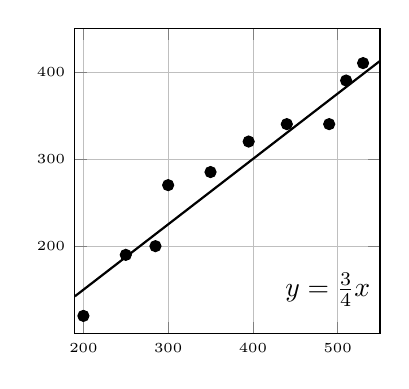
\begin{tikzpicture}
		\begin{axis}[
			ymin=100, ymax=450,
			xmin=190, xmax=550,
			xtick={200,300,400,500},
			ytick={200,300,400},	
			grid=both,
			grid style={line width=.1pt, draw=gray!10},
			major grid style={line width=.2pt,draw=gray!50},
			width=0.45\textwidth,
			height=0.45\textwidth,
			tick label style={font=\tiny}
		]
		\addplot[
			only marks,
			mark=*,
			]
			coordinates {
			(200,120) (250,190) (285,200) (300,270) (350,285) (395,320) (440,340) (490,340) (510,390) (530,410)
			};
		\addplot[
			domain=190:550, 
			samples=100, 
			thick
			]{0.75*x};
		\node[anchor=north east] at (axis cs:550,180) {$y = \frac{3}{4}x$};
		\end{axis}
	\end{tikzpicture}
\end{figure}


\begin{itemize}
	\item Dla $y = \frac23x + 30$ suma kwadratów reszt wynosi $6\,769.4$
	\item Dla $y = \frac12x + 100$  suma kwadratów reszt wynosi $14\,112.5$
	\item Dla $y = \frac34x$ suma kwadratów reszt wynosi $5\,259.4$
\end{itemize}

Zatem trzecia linia najlepiej jest dopasowana do danych spośród tej trójki

Widzimy zatem, że suma kwadratów reszt pozwala nam porównywać różne proste i ich dopasowanie do zbioru punktów. Chcielibyśmy jednak wiedzieć jak obliczyć te najlepsze parametry $a$ i $b$, a nie tylko porównywać ich szacowania. Wyprowadzenie wzorów na te parametry przekroczyłoby jednak zdecydowanie czas jaki mamy na tę prezentację :C

Prezentują się one tak
\[
	a = \frac{\sum_{i=1}^n\, y_i(x_i - \bar x)}{\sum_{i=1}^n\, (x_i - \bar x)^2}, \quad b = \bar y - \bar x a
\]

gdzie $\bar x$ i $\bar y$ to średnie arytmetyczne zmiennych $x$ i $y$.

\section{Metoda najmniejszych kwadratów w praktyce}
Skoro poznaliśmy już metodę najmniejszych kwadratów, to wykorzystajmy ją dla danych z początka prezentacji Podstawmy zatem nasze dane i wyznaczmy najlepiej dopasowaną do nich prostą!

Najpierw policzmy średnia arytmetyczne zmiennych $x$ i $y$
\[
	\bar x = \frac{1}{10} (200+250+530)=375
\]
\[
	\bar y = \frac{1}{10} (120+190+200)=286.5
\]

 Następnie obliczymy odpowiednie sumy do wzoru na współczynnik $a$
\[
	\sum_{i=1}^{10}\, y_i(x_i - \bar x) = 120 \cdot (200-375) + 190 \cdot (250-375) + ... + 410 \cdot (530-375) = 93\,675
\]
\[
	\sum_{i=1}^{10}\, (x_i - \bar x)^2 = (200-375)^2 + (250-375)^2 + ... + (530-375)^2 = 120\,700
\]

 Zostało nam już tylko podstawienie liczb do wzorów na parametry $a$ i $b$ 
\[
	a = \frac{93\,675}{120\,700} \approx 0.78
\]
\[
	b = 286.5 - 375 \cdot \frac{93\,675}{120\,700} \approx -4.54
\]

 Zatem szukana prosta jest postaci
\[
	y = 0.78x - 4.54
\]

Przedstawmy ją na wykresie razem z punktami.  Jak widzimy, prosta jest jak najbardziej dobrze dopasowana do naszych danych. Suma kwadratów reszt dla tej prostej wynosi $4\,901.5$ zatem jest o wiele mniejsza od przykładowych prostych dopasowanych “na oko” jakie rozważaliśmy wyżej.

Potwierdziło się zatem nasze przypuszczenie, że wzrostowi dochodu towarzyszy wzrost wydatków. Moglibyśmy się teraz nawet pokusić o przewidzenie jak będą wyglądały wydatki dla większych (lub mniejszych) dochodów u innych rodzin.

\section{Podsumowanie}

To tyle. W miarę prostę co nie? Podsumujmy zatem to co wiemy

\begin{itemize}
	\item Regresja liniowa to opis korelacji między zmiennymi za pomocą krzywej
	\item Dopasowanie prostej to znalezienie takich parametrów a i b, że funkcja odległości punktów pomiarowych od prostej przyjmuje wartość minimalną
	\item Metoda najmniejszych kwadratów to takie dopasowanie prostej, aby suma kwadratów różnic między punktami pomiarowymi, a prostą była jak najmniejsza
\end{itemize}

Dla zainteresowanych tematem będących ciekawych skąd wzięły się wzory na parametry a i b, wykorzystujemy tutaj optymalizację funkcji dwóch zmiennych. Znajdujemy ekstremum lokalne funkcji sumy kwadratów różnic.

%-------------------------------------------------------------------------------

\end{document}
